\section{Systembeskrivelse}
Der ønskes, som tidligere nævnt, at udvikle et system, der har til formål at støtte musklerne omkring knæleddet hos ALS-patienter under udførelse af en squat-øvelse ved anvendelse af et exoskelet. Dette gøres for at aflaste patienterne med henblik på at kunne undgå kørestol i tidlige stadier af ALS. Systemet skal kunne opsamle signaler fra quadriceps og hasemusklerne. Disse signaler skal behandles og omsættes til aktivitet, så det sammen med et programmeret system kan anvendes som en prototype af et exoskelet, som skal udføre en tilsvarende bevægelse, men også have mulighed for forstærkning af signalet, så mindre muskelkraft også vil kunne udløse denne bevægelse. Af denne grund skal systemet være i stand til at måle muskelaktivitet i quadriceps og hasemusklerne samt den aktuelle vinkel i knæleddet. Derudover skal systemet være brugervenligt ved at være kompakt, mobilt og ikke generende over for brugeren.

\subsection{Krav til systemet} 
\begin{itemize}
\item Systemet skal registrere muskelaktivitet og ledvinkler
\item Systemet skal kunne overføre data trådløst til en computer
\item Systemet skal kunne ende ud i en prototype af et exoskelet
\item Systemet skal være batteridrevet
\item Systemet skal være sikkert og ikke til gene for brugeren \fxnote{skal vi stadig skrive at det ikke skal være til gene for brugeren og er dette muligt at vurdere?}
\item Systemet skal kunne indikere, hvis der ikke er strøm nok til at virke optimalt
\end{itemize}


\subsection{Blokdiagram} \fxnote{kig på dokumentet som signe og Nirusha har lavet}
\begin{figure}[H]
\centering
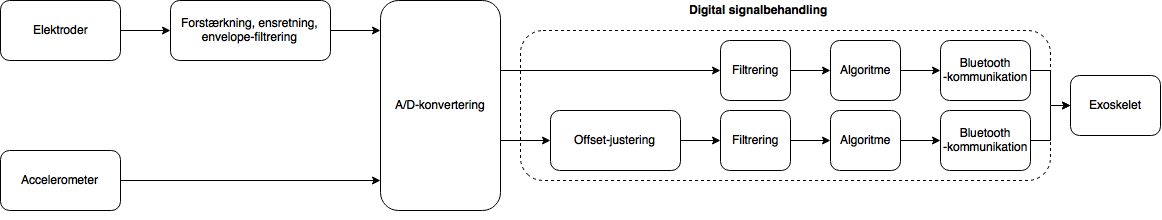
\includegraphics[width=1\textwidth]{figures/blokdiagram.png}
\caption{Systemets opbygning.}
\label{fig:blokdiagram}
\end{figure}

I dette projekt er der valgt at udarbejde en prototype, som har til formål at bøje knæleddet, når lårets muskler kontraherer. Opbygningen af systemet fremgår af \autoref{fig:blokdiagram}. Der anvendes to sensorer, EMG og accelerometer, til at opsamle biologiske signaler. For at registrere muskelaktivitet anvendes elektroder og en EMG-forstærker, der har til formål at forstærke signalet, der opsamles. Accelerometeret anvendes for at give systemet et input om, knæleddet vinkles  under udførslen af en squat-øvelse. Det opsamlede signal sendes herefter videre til den digitale del af systemet, hvilket er bestående af et Bluetooth Low Energy Pioneer kit (CY8CKIT-042-BLE), som opfanger de biologiske signaler og overfører dem trådløst til en CySmartUSB BLE Dongle sat i en computer, som kan kommunikere med prototypen af exoskelettet udarbejdet i LEGO Mindstorm. 


